\usetikzlibrary{arrows.meta}
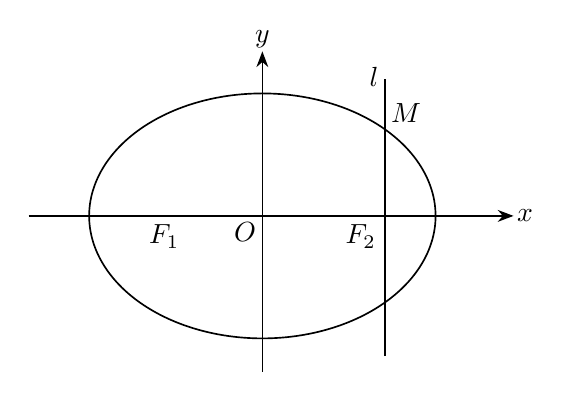
\begin{tikzpicture}[x=1.1cm,y=1.1cm,line width=.6pt,>=Stealth,font=\normalsize]
  \def\ellA{2}
  \def\ellB{1.414213562}
  \def\ellC{1.414213562}
  \coordinate (O) at (0,0);
  \coordinate (Fone) at (-1.414214,0);
  \coordinate (Ftwo) at (1.414214,0);
  \coordinate (M) at (1.414214,1);
  \draw[->] (-2.7,0) -- (2.9,0) node[right,inner sep=1pt] {$x$};
  \draw[->] (0,-1.8) -- (0,1.9) node[above,inner sep=1pt] {$y$};
  \draw[domain=0:360,samples=201,smooth,variable=\t] plot ({\ellA*cos(\t)},{\ellB*sin(\t)});
  \draw (1.414214,-1.62) -- (1.414214,1.58);
  \node[below left,inner sep=2pt] at (O) {$O$};
  \node[below right,inner sep=3pt] at (Fone) {$F_1$};
  \node[below left,inner sep=3pt] at (Ftwo) {$F_2$};
  \node[above right,inner sep=2pt] at (M) {$M$};
  \node[left,inner sep=2pt] at (1.414214,1.6) {$l$};
\end{tikzpicture}
